\begin{figure*}[th]
\centering
\fbox{\parbox{2\columnwidth}{
\sout{use
make
include
take
get
provide
show}
go
say
find
see
come
work
need
look
require
give
{\bf help}
offer
know
create
change
add
start
allow
{\bf keep}
{\bf play}
contain
run
apply
receive
call
develop
leave
begin
hold
support
cause
build
meet
increase
cover
base
want
serve
continue
{\bf read}
write
produce
{\bf bring}
involve
pay
live
ask
put
consider
set
reduce
remove
improve
appear
{\bf perform}
seem
move
lead
follow
buy
occur
try
design
contact
complete
sell
learn
determine
think
{\bf report}
describe
like
present
mean
relate
lose
feel
affect
post
represent
enjoy
send
open
discuss
{\bf visit}
enter
grow
share
maintain
identify
indicate
tell
place
list
return
choose
{\bf select}
turn
sign-up
form
obtain
stop
check
result
win
happen
install
{\bf wear}
die
love
understand
save
expect
focus
fill
watch
prevent
{\bf spend}
protect
reach
pass
raise
display
treat
ensure
{\bf connect}
achieve
establish
suggest
view
accept
associate
fit
drive
exist
control
talk
replace
deliver
avoid
hear
fall
let
{\bf define}
handle
{\bf eat}
plan
bear
prepare
manage
{\bf release}
promote
attend
experience
join
kill
seek
{\bf operate}
measure
end
refer
teach
face
conduct
explain
purchase
combine
test
{\bf cut}
generate
review
deal
break
close
reflect
decide
believe
consist
{\bf carry}
fail
collect
speak
address
encourage
match
stand
sit
stay
{\bf hit}
{\bf submit}
draw
walk
depend
limit
please
reveal
introduce
wait
arrive
enable
}}
\caption{Verb-200 (Ranked) with Verb-20 in Bold}
\label{fig:verbs}
\end{figure*}

%bring\\
%carry\\
%connect\\
%cut\\
%define\\
%eat\\
%help\\
%hit\\
%keep\\
%operate\\
%perform\\
%play\\
%read\\
%release\\
%report\\
%select\\
%spend\\
%submit\\
%visit\\
%wear\\
%\hline
%\end{tabular}
%\label{tab:verbs}
%\end{table}
%

\subsection{Dataset \& Preprocessing}
\label{sec:preprocess}
Our primary target of verb is a set of 200 most frequently used verbs in
English text\footnote{We compute the frequency of all verbs that appeared
in a very large web text corpus to obtain the 200 most frequently used
verbs. We excluded a few verbs such as ``use'', ``make'', ``get'' and
``take'' from the top of the list because they are extremely general and
have too many arguments.},
which we call Verb-200. These verbs are shown in \figref{fig:verbs}. A random
sample of 20 verbs from Verb-200 forms a smaller set of verbs called Verb-20
(highlighted in \figref{fig:verbs}) which are used in most of our experiments.
Next we create two different datasets: Web sentences and
Google syntactic N-gram data\cite{goldberg2013}\footnote{We release our dataset
 and all action concepts on \url{http://adapt.seiee.sjtu.edu.cn/~kzhu/ac}}.
The web sentence dataset, which consists of 165,758,215 English
sentences, are extracted from a crawled snapshot of web pages.
%\KZ{How many?}\textcolor{red}{[KQ:We don't know...]}
%in a snapshot of Bing's search log.
Google syntactic N-gram data is downloaded from Google Books
\footnote{http://commondatastorage.googleapis.com/books/syntactic-ngrams/index.html},
 which comprises texts from 3,473,595 English books. We use the \emph{Verbargs}
 package extracted from all the English books which consists of 130,436,458
 syntactic N-grams with verb-argument dependencies.
%\KZ{Kaiqi: We need to describe how we generate the web and
%google data sets here.
%Need to emphasize how big these data sets. Remember this ``VL''DB!}

ReVerb also provides millions of triples of predicate relation. However,
the scale of ReVerb is small to our problem. We aim at discovering
the action concepts, which needs a large number of action instances
for each verb. However, ReVerb contains small number of triples for each verb.
For example, only 374 unique triples for ``wear'' are
extracted in ReVerb while our web dataset contains 17,749 unique $<$verb, object$>$ pairs
for ``wear''. The reason of the huge different is that,
a triple must contains two arguments for the verb. However, verbs co-occur with
only one argument in many cases. Moreover, ReVerb is not only suitable to be applied for
intransitive verbs.
Intransitive verbs usually co-occur only with subject,
which is not covered by ReVerb. We do not use ReVerb data due to its limited scale.
%\KZ{We need to explain why we don't use the ReVerb data.}

%\subsection{Preprocessing of Dataset}
To make use of the web sentences and Google syntactic N-gram,
we need to preprocess the two datasets to generate action instances.

\textbf{Web Data} is a set of plain texts extracted from web pages.
We run a dependency parser on the whole corpus and
store the dependency tree for each sentence. The result of
dependency parsing contains relation between verb-subject and
verb-object. The head word of subject is usually labeled
as ``nsubj'' while the head word object is usually
labeled as ``dobj'' or ``nsubjpass''.
We can retrieve the phrase of subject or object in the dependency
tree by returning the whole subtree rooted on the head.
However, the whole phrase of subject/object is not always
a Probase term. As shown in \figref{fig:pterm},
the phrase ``a flashy baseball cap''
is extracted as the object of ``wear''. However,
the whole phrase is not a valid Probase term.
To make use of the knowledge base, we need to
detect Probase term from the subject/object phrase(e.g. baseball cap).

\begin{figure}[th]
\centering
\epsfig{file=pterm.eps,width=\columnwidth}
\caption{Dependency Parse Tree}
\label{fig:pterm}
\end{figure}

We use a sliding window strategy to extract longest
Probase term that we can detect in the whole phrase.
We keep a sliding window slides around the head word
from right to left,
and check if there is a Probase term satisfied.
The initial size of the window is the length of the
whole phrase. If we detect a Probase term,
we return the phrase captured in the window;
Otherwise, we decrease the window size and slides
around the head term again. We stop until we find
any Probase term. Usually, this procedure can detect
a Probase term from the phrase, because Probase includes
most of the words(phrase with length 1). After
preprocessing, we output all the pairs of verb-subject and
verb-subject as action instances.

\begin{table}[th]
\centering
%\scriptsize
\caption{Snapshot of Google Syntactic N-gram}
\begin{tabular}{|l|l|}
\hline
Verb & N-gram \\
\hline \hline
accept & firms/NNS/nsubj/2\; accept/VBP/conj/0\; \\
& money/NN/dobj/2\; in/IN/prep/2\; \\
& exchange/NN/pobj/4   \\
\hline
delay & to/TO/aux/2\; delay/VB/xcomp/0\; \\
& these/DT/det/4\; matters/NNS/dobj/2 \\
\hline
spent & an/DT/det/2\; afternoon/NN/nsubjpass/4\; \\
& was/VBD/aux/4\; spent/VBN/conj/0\\
\hline
\end{tabular}
\label{tab:ngram}
\end{table}

\textbf{Google syntactic n-gram} contains
relations between verbs and arguments. A snapshot
of Google syntactic n-gram is shown in \tabref{tab:ngram}.
The syntactic n-gram consist of the dependency parsing
result conducted by Stanford parser. Each token is
labeled with POS tag, dependency and head index(the number
at the end of each token). To apply this data
to our task, we need to detect the subjects and objects
from the n-gram. First, we restore the n-gram to the dependency
according to the head index. Second, we find head of the
subject or object from the nodes that directly connect to
the verb node with the dependency label ``nsubj'', ``dobj''
or ``nsubjpass''. Around the head, we use the same sliding window
algorithm to find a longest Probase term to be the subject/object
as in the processing of the web data. Also, we restore the
tense of the verb to the present tense.
After these processings, the data becomes two lists of pairs
in the form of $<$verb, subject$>$ and $<$verb, object$>$, respectively.


